\section{Load balance}
\tikzstyle{vertex}=[auto=left,circle,fill=black!25,minimum size=20pt,inner sep=0pt]

\begin{itemize}
	\item \textbf{Description:} \\
		Let $x_i, i = 1,2,..., N;y_k, k = 1,2,...,M$ represent the nodes of jobs and computers respectively, add two nodes $s$ and $t$, construct a initial network like this 
	\begin{center} 
	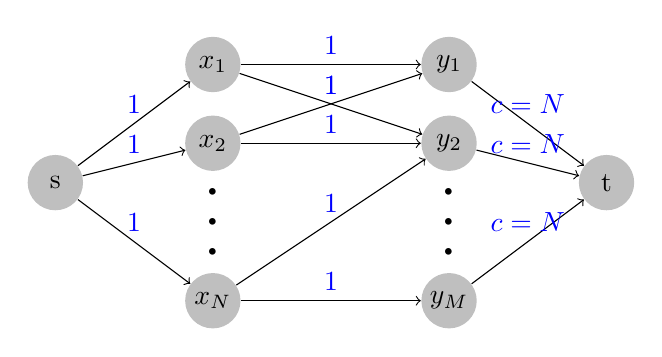
\begin{tikzpicture}
	\node[vertex] (s)  at (1,4.5)  {s};
	\node[vertex] (x1)  at (3,6)  {$x_1$};
	\node[vertex] (x2)  at (3,5)  {$x_2$};
	\node[vertex] (xn)  at (3,3)  {$x_N$};
	
	\node[vertex] (t)  at (8,4.5)  {t};
	\node[vertex] (y1)  at (6,6)  {$y_1$};
	\node[vertex] (y2)  at (6,5)  {$y_2$};
	\node[vertex] (ym) at (6,3)  {$y_M$};
	
	\path (x2) -- (xn) node [black, font=\Huge, midway, sloped] {$\dots$};
	\path (y2) -- (ym) node [black, font=\Huge, midway, sloped] {$\dots$};

	\foreach \from/\to/\weight in {s/x1/1, s/x2/1,  s/xn/1,
		x1/y1/1, x1/y2/1, x2/y1/1, x2/y2/1, xn/y2/1, xn/ym/1}
	\draw[->] (\from) -- (\to) node [midway, above, blue] {$\weight$};
 
	\foreach \from/\to/\weight in {y1/t/c=N, y2/t/c=N, ym/t/c=N}
	  \draw [->] (\from) -- (\to) node [midway, above, blue] {$\weight$};
	\end{tikzpicture}
	\end{center} 
	we can find a flow of maximum value $val(f)$ using method like FORD-FULKERSON ,
	if $val(f)$ is exactly the number of jobs $N$, then we reduce each capacity $c$ from $y_i$ to $t$,   if we still get $val(f) = N$, we can continue to reduce the capacity $c$;
	otherwise, we should increase the capacity.If we can not reduce the capacity $c$
	to maintain $val(f) = N$, then we get the max load.
	Binary search can be used to adjust the capacity.  
		
	\item \textbf{Correctness:} \\
		 Since we must maintain the maximum flow value $val(f)$ equals to the number of jobs $N$,
		 the max load is no larger than the capacity $c$, reduce the capacity $c$ until $val(f)$ not 
		 equals $N$,then the capacity $c$ is the minimum max load.
	\item \textbf{Complexity:} 
		\begin{itemize}
			\item FORD-FULKERSON costs $O((3N+M)^2(N+M+2))$ time using Edmonds-karp
			\item binary search averagely costs $O(\log N)$ time
		\end{itemize}
		In summary , it costs $O(\log N (3N+M)^2(N+M+2))$ time
		\begin{algorithm}[H]
			\caption{load balance}
			\begin{algorithmic}[1]
				\Require  the number of jobs and two computer ID for each job 
				\Ensure   minimum of the max load	
				\Function {load-balance} {}
				\State add two nodes $s$ and $t$,construct the initial network $G$ 
				\State set each capacity $c$  with $N$
				\State left = $0$, right = $N$
				\State max\_load = N, pre\_load = $N$
				\While {left <= right}
				\State pre\_load = max\_load
				\State max\_load = left + (right-left)/2
				\State set the capacity $c$ with max\_load 
				\State max\_flow = FORD-FULKERSON($s$,$t$)
				\If {max\_flow = $N$}
				\State right = max\_load - 1
				\Else
				\State left = max\_load + 1
				\EndIf 	
				\If {left >= right and max\_flow $\neq N$}
				\State max\_load = pre\_load
				\EndIf	  
				\EndWhile
				\State \Return max\_load 				 
				\EndFunction 
			\end{algorithmic} 
		\end{algorithm}	
\end{itemize}
 